\subsection{Contact Estimation with Ultrasound Image}
For each ultrasound frame $j$, a confidence map $C_j(u,v)\in[0,1]$ is computed using the random-walk method~\cite{Karamalis2012}.
Following~\cite{welleweerd2021out}, a shallow near-field region is used to characterize acoustic coupling along the probe aperture while reducing the influence of deeper anatomy.
The confidence map is averaged along depth to form a lateral profile $\bar C_j(u)$, which is divided into $N$ equal-width regions, yielding $\mathbf c_j=[c_{1,j},\ldots,c_{N,j}]^\top$.
A bin with $c_{i,j}<c_{\mathrm{th}}$ is treated as poorly coupled (insufficient acoustic contact) on that portion of the aperture.
Fig.~\ref{fig:USCON} shows one frame of this procedure on a $50\times50$~mm field: $u$ is lateral from the probe-face centre and $v$ is depth from the face into tissue.
We use $N=10$ and mark $c_{i,j}<c_{\mathrm{th}}$ in red ($c_{\mathrm{th}}=0.8$).

\begin{figure}[t]
\centering
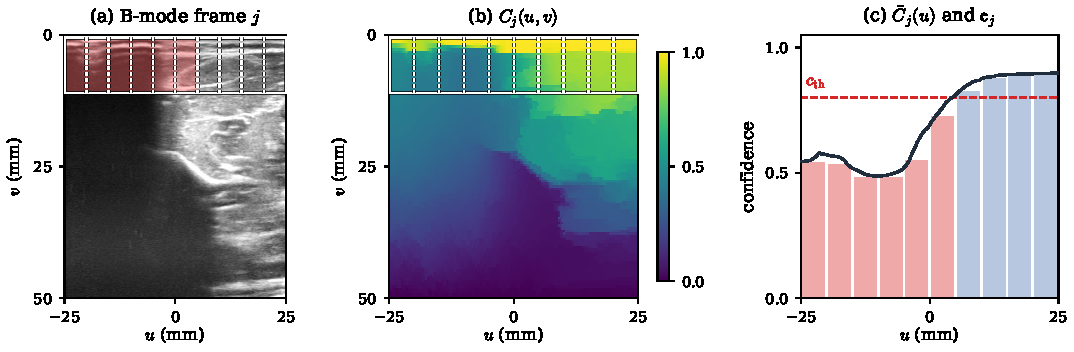
\includegraphics[width=\columnwidth]{USCON}
\caption{Contact estimation from one ultrasound frame.
(a)~B-mode with the near-field ROI (box) and $N$ equal-width bins (dashed); $u\in[-25,25]$~mm, $v\in[0,50]$~mm.
(b)~Confidence $C_j(u,v)$.
(c)~Lateral profile $\bar C_j(u)$ (curve) and $\mathbf c_j$ (bars).
Red: $c_{i,j}<c_{\mathrm{th}}$ (poor coupling).}
\label{fig:USCON}
\end{figure}
